\documentclass[11pt]{article}
\usepackage[utf8]{inputenc}
\usepackage[T1]{fontenc}
\usepackage{geometry}
\usepackage{graphicx}
\usepackage{fancyhdr}
\usepackage{parskip}
\usepackage{url}
\usepackage{float}
\usepackage{caption}
\usepackage{tabularx}
\usepackage{longtable}
\usepackage{booktabs}
\usepackage{array}
\usepackage{listings}
\usepackage{xcolor}
\usepackage{xspace}
\usepackage{tikz}
\usetikzlibrary{arrows.meta, positioning, shapes.geometric, fit}
\captionsetup{font=it}
\captionsetup{justification=centering}

\geometry{margin=1in}
\emergencystretch=2em
\setlength{\headheight}{42pt}
\pagestyle{fancy}
\fancyhf{}
\fancyhead[R]{
\includegraphics[height=0.5in]{../artifacts/logo.png}}
\fancyfoot[C]{\thepage}
\renewcommand{\headrulewidth}{0pt}

\lstset{
  basicstyle=\ttfamily\footnotesize,
  breaklines=true,
  columns=fullflexible,
  frame=single,
  framerule=0.3pt,
  xleftmargin=0pt,
  aboveskip=0.5em,
  belowskip=0.5em,
  showstringspaces=false
}

\newcommand{\todo}[1][]{\textit{[TODO\ifx\relax#1\relax\else: #1\fi]}\xspace}
\newcommand{\pass}{\textbf{Pass:}\ }
\newcommand{\prop}{\textsuperscript{$\dagger$}}

% Block styles for the diagrams
\tikzset{
  box/.style={draw, rounded corners=2pt, align=center, font=\footnotesize, inner sep=4pt, minimum height=0.8cm, fill=gray!8},
  dec/.style={draw, diamond, aspect=2.4, align=center, font=\scriptsize, inner sep=1pt, fill=gray!8},
  arr/.style={-{Stealth[length=2mm]}, thick},
  lbl/.style={font=\scriptsize, fill=white, inner sep=1.5pt, outer sep=3pt, align=center}
}

\begin{document}
\begin{titlepage}
  \centering
  \vspace*{1in}
  {\fontsize{25pt}{30pt}\selectfont\textbf{T2: Beta Test Plan}\par}
  \vspace{0.5in}
  {\LARGE\textbf{EEL4908 CpE Design 2}\par}
  \vspace{0.35em}
  {\Large Hardened RISC-V Exam Computer\par}
  \vspace{0.3em}
  {\Large October 1, 2026\par}
  \vspace{0.6in}
  {\Large Cannon Spencer \quad George Rushevich \quad Justin Reyes \quad Gabriel Velazquez\par}
  \vspace{1in}
  
\includegraphics[height=1.65in]{../artifacts/uf-logo.png}\hspace{1.25in}%
  
\includegraphics[height=1.65in]{../artifacts/big-logo.png}\par
\end{titlepage}
\newpage
\setcounter{page}{1}


%=============================================================================
\section{Scope}
%=============================================================================

\textbf{Beta objective.} Two boards accept a ``start SEB'' command from the server, and SEB launches on both.

Repository: \url{https://github.com/cannon-spencer/riscv-exam-computer}. Commit tested: \todo

\paragraph{In scope.} Control server, board agent, start and stop scripts, SEB session on the board. \todo (add or remove items)

\paragraph{Out of scope.} \todo

\paragraph{Notation.} \todo marks something for the team to fill in or confirm; where the blank is not obvious, a short note after the colon says what to write. Nothing marked TODO has been measured or decided.

%=============================================================================
\section{Alpha test results}
%=============================================================================

Describe the results of the alpha testing, how they changed the project, and how they influenced this plan. In the table below, give each test a result (Pass, Fail or Not run) and note the evidence.

\subsection{Results against the T1 plan}

\begin{longtable}{@{}p{0.11\textwidth}p{0.17\textwidth}p{0.67\textwidth}@{}}
\toprule
\textbf{T1 ID} & \textbf{Result} & \textbf{Evidence and notes} \\
\midrule
\endhead
HW-01 & \todo & \todo \\
HW-02 & \todo & \todo \\
HW-03 & \todo & \todo \\
SW-01 & \todo & \todo \\
INT-01 & \todo & \todo \\
INT-02 & \todo & \todo \\
SW-02 & \todo & \todo \\
\bottomrule
\caption{Alpha results.}\label{tab:alpha}
\end{longtable}

\subsection{How alpha testing changed the project}

\todo[for each alpha finding, say what you saw and what you changed]

\subsection{How alpha testing shaped this plan}

\todo[for each alpha finding, give the beta test ID that checks it]

%=============================================================================
\section{Expected behavior}
%=============================================================================

This section describes behavior as implemented in the source at the tested commit.

\subsection{System overview}

\begin{figure}[H]
  \centering
  \begin{tikzpicture}[x=1cm, y=1cm]
    \node[box] (inst) at (0,0) {Instructor\\\texttt{curl}};
    \node[box] (srv) at (5.2,0) {Control server\\port 8000, in-memory\\inventory};
    \node[box, minimum width=5.4cm] (cf) at (11.2,0) {Cloudflare tunnel\\\texttt{riscv-exam-computer.download}};
    \node[box] (ba) at (9.5,-2.7) {Board A\\\texttt{seb-agent}};
    \node[box] (bb) at (13.1,-2.7) {Board B\\\texttt{seb-agent}};
    \node[box] (sa) at (9.5,-5.2) {\texttt{start-seb.sh}\\xinit, openbox, SEB};
    \node[box] (sb) at (13.1,-5.2) {\texttt{start-seb.sh}\\xinit, openbox, SEB};

    \draw[arr] (inst) -- node[lbl, above] {\texttt{POST /start}} (srv);
    \draw[arr, <->] (srv) -- node[lbl, above] {HTTP} (cf);
    \draw[arr, <->] (ba.north) -- node[lbl, left] {HTTPS heartbeat,\\reply may carry\\a job} (ba.north |- cf.south);
    \draw[arr, <->] (bb.north) -- (bb.north |- cf.south);
    \draw[arr] (ba) -- node[lbl, left] {\texttt{sudo -n}} (sa);
    \draw[arr] (bb) -- node[lbl, right] {\texttt{sudo -n}} (sb);
  \end{tikzpicture}
  \caption{Control path. Boards poll the server; the server never connects to a board.}
  \label{fig:arch}
\end{figure}

\subsection{Control server}

The server (\path{exam-env/server/src/main.rs}) listens on port 8000 and holds, per host name, the last heartbeat time, the last reported state and at most one pending job (\texttt{start} or \texttt{stop}).

\begin{table}[H]
  \centering
  \footnotesize
  \begin{tabularx}{\textwidth}{@{}l X@{}}
    \toprule
    \textbf{Route} & \textbf{Expected behavior} \\
    \midrule
    \texttt{POST /heartbeat} &
    Body \texttt{\{"host":\ldots,"state":\ldots\}}. Records the host, time and state. Replies \texttt{\{"ok":true,"job":\ldots\}} where \texttt{job} is \texttt{"start"}, \texttt{"stop"} or \texttt{null}. Missing \texttt{host}: 422. Invalid JSON: 400. No JSON content type: 415. \\
    \texttt{GET /machines} &
    Lists every host seen since the server started, with \texttt{state}, \texttt{pending} and \texttt{seen\_secs\_ago}, sorted by host. \\
    \texttt{POST /start} &
    Sets pending \texttt{start} on every host whose last heartbeat is 15\,s old or less, and returns the sorted list \texttt{queued}. Returns \texttt{"queued":[{}]} when no host is online. \\
    \texttt{POST /stop} &
    Same as \texttt{/start} with job \texttt{stop}. \\
    \bottomrule
  \end{tabularx}
  \caption{Server routes.}
  \label{tab:routes}
\end{table}

Job delivery rules (checked by SRV-01 to SRV-09):
\begin{itemize}\setlength{\itemsep}{0.12em}
  \item A job is handed out in the reply to the board's next heartbeat and then cleared.
  \item A pending \texttt{start} is not delivered while the board reports \texttt{running}; it stays pending and is delivered the first time the board reports another state.
  \item A pending \texttt{stop} is delivered regardless of reported state.
  \item There is one pending slot per board, so a later command replaces an earlier undelivered one.
  \item Inventory is held in memory only.
\end{itemize}

\subsection{Board agent}

\begin{figure}[H]
  \centering
  \begin{tikzpicture}[scale=0.8, transform shape, box/.append style={text width=4.4cm}]
    \node[box] (st) at (0,0) {Report state: \texttt{running} if the SEB child is alive, else \texttt{idle}};
    \node[box] (po) at (0,-1.9) {POST heartbeat to the control URL};
    \node[dec] (jb) at (0,-3.9) {reply\\\texttt{job}?};
    \node[box] (sl) at (0,-6.3) {Sleep 5\,s};
    \node[box] (er) at (-7.1,-1.9) {On error: log \texttt{heartbeat failed}};
    \node[box] (sa) at (6.6,-2.9) {\texttt{start}: if no live child, \texttt{sudo -n \~{}/start-seb.sh}};
    \node[box] (sp) at (6.6,-4.9) {\texttt{stop}: \texttt{sudo -n \~{}/stop-seb.sh}, then reap the child};

    \draw[arr] (st) -- (po);
    \draw[arr] (po) -- node[lbl, right] {reply received} (jb);
    \draw[arr] (po) -- node[lbl, above] {request fails} (er);
    \draw[arr] (er.south) |- (sl.west);
    \draw[arr] (jb.south) -- node[lbl, right] {\texttt{null}} (sl.north);
    \draw (jb.east) -- (2.9,-3.9);
    \draw (2.9,-2.9) -- (2.9,-4.9);
    \draw[arr] (2.9,-2.9) -- node[lbl, above] {\texttt{start}} (sa.west);
    \draw[arr] (2.9,-4.9) -- node[lbl, above] {\texttt{stop}} (sp.west);
    \draw (sa.east) -- (9.8,-2.9) -- (9.8,-6.3);
    \draw (sp.east) -- (9.8,-4.9);
    \draw[arr] (9.8,-6.3) -- (sl.east);
    \draw[arr] (sl.south) -- (0,-7.2) -| (-10.1,0) -- (st.west);
  \end{tikzpicture}
  \caption{Agent loop (\texttt{exam-env/seb-agent/src/main.rs}).}
  \label{fig:agent}
\end{figure}

\begin{itemize}\setlength{\itemsep}{0.12em}
  \item The agent heartbeats every 5\,s (sleep between requests) and reports \texttt{running} while the SEB child process it started is alive, otherwise \texttt{idle}.
  \item The reported host name is the \texttt{HOSTNAME} environment variable, set by the systemd unit from the \texttt{\%H} specifier.
  \item The control URL is compiled into the agent: \path{https://riscv-exam-computer.download/heartbeat}.
  \item The agent opens no listening port.
  \item Sudo for the agent is limited to \path{/home/orangepi/start-seb.sh} and \path{/home/orangepi/stop-seb.sh}.
\end{itemize}

\subsection{Board session}

\paragraph{Start.} \texttt{start-seb.sh} runs as root and execs \texttt{xinit} on display \texttt{:1}, virtual terminal 3, starting \texttt{openbox} and then \texttt{\~{}/safe-exam-browser -{}-windowed \~{}/demo-exam.json}.

\paragraph{Stop.} \texttt{stop-seb.sh} kills the SEB and \texttt{xinit} processes and X1 socket holders, rebinds the framebuffer console, restores keyboard mode and switches to virtual terminal 1.

\subsection{Quantified requirements}

\begin{table}[H]
  \centering
  \footnotesize
  \begin{tabularx}{\textwidth}{@{}l X l@{}}
    \toprule
    \textbf{ID} & \textbf{Requirement} & \textbf{Value} \\
    \midrule
    R-T1 & Heartbeat sleep between requests & 5\,s (code) \\
    R-T2 & A board counts as online while its last heartbeat is no older than & 15\,s (code) \\
    R-T3 & Time from \texttt{POST /start} to SEB running on every online board, in seconds & \todo \\
    R-T4 & Maximum difference between the two boards' start times, in seconds & \todo \\
    R-T5 & Time from \texttt{POST /stop} to console restored, in seconds & \todo \\
    R-P1 & Canvas page load time, in seconds & \todo \\
    R-P2 & Click-to-response latency in Canvas, in seconds & \todo \\
    R-P3 & Maximum board temperature during a session, in \textdegree{}C & \todo \\
    \bottomrule
  \end{tabularx}
  \caption{Quantified requirements. Rows marked TODO are to be set by the team.}
  \label{tab:req}
\end{table}

\subsection{Not implemented in the tested commit}

\begin{itemize}\setlength{\itemsep}{0.12em}
  \item The server code has no authentication on any route.
  \item \texttt{/start} and \texttt{/stop} address all online boards; there is no per-board targeting.
  \item The server does not send configuration to boards; the agent starts SEB with a local config file.
  \item Secure start (the exam opening only under SEB): \todo[describe what should happen, and how it would be tested]
  \item Other: \todo
\end{itemize}

%=============================================================================
\section{Test procedures}
\label{sec:proc}
%=============================================================================

\subsection{Equipment and conventions}

\todo[list the boards, displays, laptop, network and tools you actually use] Record the commit and board names for every run in Table~\ref{tab:log}.

\subsection{Server (no hardware)}

Run \path{./scripts/test-server-api.sh} against a freshly started local server (\texttt{SLOW=1} adds SRV-09). Do not point it at a server that live boards are using.

\begin{longtable}{@{}p{0.115\textwidth}p{0.835\textwidth}@{}}
\toprule
\textbf{ID} & \textbf{Procedure and pass criterion} \\
\midrule
\endhead
SRV-01 & \textbf{Heartbeat.} POST a heartbeat for a new host. \pass reply contains \texttt{"ok":true} and \texttt{"job":null}. \\
SRV-02 & \textbf{Inventory.} Heartbeat two hosts, then \texttt{GET /machines}. \pass both hosts listed with state and \texttt{seen\_secs\_ago}. \\
SRV-03 & \textbf{Broadcast start.} \texttt{POST /start} with both hosts online. \pass \texttt{queued} lists both; the next heartbeat from a host returns \texttt{start}, the one after returns \texttt{null}. \\
SRV-04 & \textbf{Start withheld while running.} Heartbeat with state \texttt{running} while \texttt{start} is pending. \pass no job returned and \texttt{/machines} still shows \texttt{pending:"start"}. \\
SRV-05 & \textbf{Stop always delivered.} \texttt{POST /stop}, then heartbeat from a running and an idle host. \pass both receive \texttt{stop}. \\
SRV-06 & \textbf{Single slot.} \texttt{/start} then \texttt{/stop} before the board polls. \pass only \texttt{stop} is delivered. \\
SRV-07 & \textbf{Pending start after exit.} \texttt{/start} while running, then report \texttt{idle}. \pass \texttt{start} is delivered. \\
SRV-08 & \textbf{Bad input.} Missing host, invalid JSON, no content type, \texttt{GET /start}. \pass 422, 400, 415, 405, and \texttt{/machines} still answers 200. \\
SRV-09 & \textbf{Offline exclusion.} Stop heartbeating for 16\,s, then \texttt{POST /start}. \pass \texttt{"queued":[{}]}. \\
\bottomrule
\caption{Server tests.}\label{tab:srv}
\end{longtable}

\subsection{Agent and board}

\begin{longtable}{@{}p{0.115\textwidth}p{0.835\textwidth}@{}}
\toprule
\textbf{ID} & \textbf{Procedure and pass criterion} \\
\midrule
\endhead
INS-01 & \textbf{Fresh install.} Flash a card, run \texttt{install-software.sh} and \texttt{install-seb.sh} with \texttt{-{}-host}, then any manual steps. Record every manual step needed. \pass \texttt{systemctl -{}-user is-active seb-agent} prints \texttt{active}, \path{~/safe-exam-browser} exists and is executable, and the board appears in \texttt{/machines}. \\
AGT-01 & \textbf{Unique identity.} On each board run \texttt{hostname} and \texttt{systemctl -{}-user show seb-agent -p Environment}. \pass \texttt{/machines} lists each board as a separate host. \\
AGT-02 & \textbf{Cadence.} \texttt{journalctl -{}-user -u seb-agent -o short-precise -n 25}. \pass intervals match R-T1; acceptable range \todo. \\
AGT-03 & \textbf{Outage tolerance.} Make the control URL unreachable for a set time, then restore it. \pass the agent keeps running, logs each failed heartbeat, and resumes heartbeating after restoration; duration and recovery time \todo. \\
AGT-04 & \textbf{Agent crash recovery.} Kill the agent process. \pass the systemd unit restarts it; time limit \todo. \\
AGT-05 & \textbf{Boot without login.} Power-cycle a board and do not log in. \pass the board is listed in \texttt{/machines}; time limit \todo. \\
SUDO-01 & \textbf{Sudo scope.} As \texttt{orangepi} run \texttt{sudo -n -l}. \pass only the two scripts are listed. \\
SES-01 & \textbf{Start from console.} Run \texttt{sudo -n \~{}/start-seb.sh}. \pass SEB is visible on the display; time limit \todo. \\
SES-02 & \textbf{Stop from console.} Run \texttt{sudo -n \~{}/stop-seb.sh}. \pass no SEB or \texttt{xinit} process remains, the text console is shown and the keyboard works. \\
SES-03 & \textbf{Repeated cycles.} Start and stop repeatedly, recording memory use each cycle. \pass every cycle meets SES-01 and SES-02; number of cycles and memory tolerance \todo. \\
SES-04 & \textbf{Duplicate start.} While running, send \texttt{POST /start} twice. \pass a single SEB session. \\
SES-05 & \textbf{Config.} Validate \path{~/demo-exam.json} and read its start URL. \pass valid JSON, SEB starts without a password prompt; expected start URL \todo. \\
\bottomrule
\caption{Agent and board session tests.}\label{tab:agent}
\end{longtable}

\subsection{Integration and demo}

\begin{longtable}{@{}p{0.115\textwidth}p{0.835\textwidth}@{}}
\toprule
\textbf{ID} & \textbf{Procedure and pass criterion} \\
\midrule
\endhead
DEMO-01 & \textbf{Two boards start and stop on one command.}
Pre: SES-01, SES-02 and AGT-01 passed on both boards; both listed \texttt{idle} in \texttt{/machines}.
Steps: (1) note the time; (2) \texttt{curl -sS -X POST \$CTRL/start}; (3) record when SEB appears on each display; (4) \texttt{GET /machines}; (5) \texttt{curl -sS -X POST \$CTRL/stop}; (6) record when each display returns to the console. Number of trials \todo.
\pass \texttt{queued} lists both boards; SEB runs on both; \texttt{/machines} shows both \texttt{running}; after stop both are back at the console. Time limits R-T3 to R-T5 \todo. \\
DEMO-02 & \textbf{Board offline at start.} Stop one board's agent, send \texttt{POST /start}. \pass \texttt{queued} lists only the other board. Restart the agent; record whether it launches SEB. Send \texttt{/start} again and record the result. \\
DEMO-03 & \textbf{Board loses network while running.} With both running, disconnect one board. Record SEB state, the board's \texttt{seen\_secs\_ago}, and the \texttt{queued} list for a \texttt{POST /stop}. Reconnect and send \texttt{/stop} again. \\
DEMO-04 & \textbf{Server restart.} With both boards running, restart the server. Record how long until both are listed again and with which state. \\
EDGE-01 & \textbf{Pending start after self-exit.} While a board runs, send \texttt{/start}, then end SEB locally. Record whether SEB relaunches. Decide whether that is intended. \\
\bottomrule
\caption{Integration and demo tests.}\label{tab:demo}
\end{longtable}

\subsection{Lockdown and security}

\begin{longtable}{@{}p{0.115\textwidth}p{0.835\textwidth}@{}}
\toprule
\textbf{ID} & \textbf{Procedure and pass criterion} \\
\midrule
\endhead
LD-01 & \textbf{Exit paths.} With SEB started by the agent, try the key combinations, mouse actions and window actions the team lists here: \todo. \pass none gives a shell, another application or the console. Record each attempt and outcome. \\
SEC-01 & \textbf{Secure start.} \todo[write what secure start should mean and how to test it]. \\
SEC-02 & \textbf{No inbound surface.} On a board run \texttt{ss -ltnp}. \pass no listening socket belongs to \texttt{seb-agent}. \\
SEC-03 & \textbf{Control-channel access.} Record whether \texttt{POST /start} and \texttt{POST /stop} succeed from a machine with no credentials, with no exam running. \\
\bottomrule
\caption{Lockdown and security tests.}\label{tab:sec}
\end{longtable}

\subsection{Performance and endurance}

\begin{longtable}{@{}p{0.115\textwidth}p{0.835\textwidth}@{}}
\toprule
\textbf{ID} & \textbf{Procedure and pass criterion} \\
\midrule
\endhead
PERF-01 & \textbf{Page load.} Start SEB with \texttt{/start}; time the Canvas pages the team lists: \todo. Number of runs \todo. Report median and maximum. \pass R-P1. \\
PERF-02 & \textbf{Input latency.} Time click to visible response over a set number of clicks \todo. \pass R-P2. \\
PERF-03 & \textbf{Thermal.} Run a Canvas session of set length \todo\ while logging temperature at a set interval \todo (log method \todo). \pass R-P3. \\
PERF-04 & \textbf{Endurance.} Run SEB for a set duration \todo. Count crashes, agent restarts and display glitches. \pass counts and limits \todo. \\
\bottomrule
\caption{Performance tests.}\label{tab:perf}
\end{longtable}

\subsection{Demo runbook (DEMO-01)}

\begin{lstlisting}
# laptop: start server and tunnel (Docker running)
./scripts/deploy-server.sh

# second terminal
CTRL=https://riscv-exam-computer.download
curl -sS $CTRL/machines          # both boards listed, state idle
curl -sS -X POST $CTRL/start     # queued lists both boards
curl -sS $CTRL/machines          # both boards state running
curl -sS -X POST $CTRL/stop      # both boards back at the console
\end{lstlisting}

%=============================================================================
\section{Traceability}
%=============================================================================

\begin{table}[H]
  \centering
  \footnotesize
  \begin{tabularx}{\textwidth}{@{}p{0.46\textwidth}X@{}}
    \toprule
    \textbf{Expected behavior} & \textbf{Tests} \\
    \midrule
    Server routes and job rules & SRV-01 to SRV-09, EDGE-01 \\
    Agent loop, identity, recovery & AGT-01 to AGT-05, SUDO-01, INS-01 \\
    Board session start and stop & SES-01 to SES-05 \\
    Two-board start and stop (beta objective) & DEMO-01 to DEMO-04 \\
    Timing requirements & AGT-02, DEMO-01, SES-01, SES-02 \\
    Performance requirements & PERF-01 to PERF-04 \\
    Lockdown and security & LD-01, SEC-01 to SEC-03 \\
    Alpha findings & \todo \\
    \bottomrule
  \end{tabularx}
  \caption{Expected behavior to tests.}
  \label{tab:trace}
\end{table}

%=============================================================================
\section{Results record}
%=============================================================================

\begin{table}[H]
  \centering
  \footnotesize
  \setlength{\tabcolsep}{3pt}
  \begin{tabularx}{\textwidth}{@{}p{0.08\textwidth}p{0.11\textwidth}p{0.10\textwidth}p{0.10\textwidth}p{0.09\textwidth}X@{}}
    \toprule
    \textbf{Test} & \textbf{Date} & \textbf{Tester} & \textbf{Boards} & \textbf{Result} & \textbf{Measurements and notes} \\
    \midrule
    \rule{0pt}{2.2em} & & & & & \\
    \rule{0pt}{2.2em} & & & & & \\
    \rule{0pt}{2.2em} & & & & & \\
    \rule{0pt}{2.2em} & & & & & \\
    \bottomrule
  \end{tabularx}
  \caption{Results record template.}
  \label{tab:log}
\end{table}

\end{document}
